\section{Cover decidability}
\label{sec:cover-decidability}

\subsection{Set-up}
\label{sec:decidability-set-up}

\ifintuition
\subsection{Intuition}

Our aim is to prove the decidability of the coverability problem for BNRA which can only send a single value in each broadcast. The constructions will actually lead us to a decidability proof for specifications of two different types, both subsuming the coverability specification.

\paragraph*{Step 1 : simplification} In Lemma~\ref{lem:simple-reduction} we prove that all protocols, even those which can apply several operations when receiving a broadcast, can be simulated by a protocol with a single operation upon reception of a message and no $*$ operation. A previous lemma already allowed us to remove $\diseqtestact$, thus we only have to prove decidability for systems with one operation per reception and only $\enregact$ and $\eqtestact$ operations.

Lemma~\ref{lem:simple-reduction} is placed within the decidability proof as the constructions defined there may simplify the proof of the lemma (they allow us to prove that BRNA can simulate each other simply by proving that their local runs have the same behaviour).

\paragraph*{Step 2 : run decomposition} Say we have a global run $\rho$ in which an agent broadcasts a message $m_f$. We isolate the local run $u$ of the first agent $a$ broadcasting $m_f$.
In order to execute $u$, we need to receive a sequence of broadcast that matches the sequence of receive transitions in $u$. Let $v$ be a value appearing in $u$.

\begin{itemize}
	\item 
	Say $v$ is not an initial value of $u$, let $w \in \messages^*$ be the sequence of broadcasts received by $a$ with value $v$ in $u$. Then the exact value $v$ does not matter, all $a$ needs is to receive a sequence of broadcasts with the messages of $w$ all with the same value. This is possible if and only if there exists a global run $\run'$ and a value $v'$ such that $w$ is a subword of the sequence of broadcasts made in that run with value $v'$. Indeed, if there exists such a run, then $u$ can receive selected broadcasts from $\rho'$ (happening in parallel) in order to get the sequence $w$ of messages with the same value. Conversely, if $u$ receives a sequence $w$ all with the same value in $\rho$, then the prefix of $\rho$ ending just before the broadcast of $m_f$ by $u$ is a fitting candidate for $\rho'$.
	We do not take $\rho$ directly as witness as we want the runs to get shorter as we make the recursive calls.
	
	Here we have our first type of specification, given as a word $w \in \messages^*$. We ask that there exists a global run and a value $v'$ such that $w$ is a subword of the sequence of broadcasts made in the global run with value $v'$.
	
	
	\item 	
	Now suppose $v$ is an initial value of $u$. This situation is very different as other processes need $a$ to send some messages with this value in order to be able to send it back to him.
	The key observation is that once an agent $a'$ other than $a$ has managed to broadcast some message $m$ with value $v$, we have an unlimited supply of such broadcasts:
	Let $w$ be the sequence of messages broadcast by $a$ with value $v$ before $a'$ makes that broadcast, we now know that there is a global run which, if presented with an external sequence of messages $w$ with the same value, can then broadcast $m$ with that value.
	We then extend this reasoning and consider the sequence of broadcast made with value $v$ through $\run$. It can be decomposed as  $(w_0, m_1, w_1, \ldots, m_\ell, w_\ell)$ where $w_0 \cdots w_\ell$ is the sequence of broadcasts made by $a$ with that value and the $m_j$ are placed at the moments where another agent manages for the first time to broadcast that message (from then on we have unlimited supplies of broadcasts with that value and message $m_j$). In particular $\ell \leq \size{\messages}$.
	
	All we have to do is to check for all $j$ that there exists a global run in which some agent broadcasts $m_j$ with a value $v$ that is not one of its initial ones, while having received a sequence of external messages $w'$ which is of the form $w'_0\cdots w'_{j-1}$ where each $w'_i$ is obtained by adding some letters from $\set{m_0, \ldots, m_i}$ in $w_i$.
	If we have such a run, then with the copycat property we can add an  agent that copies 
	
	This forms our second type of specification, given by a decomposition $(w_0, m_1, w_1, \ldots, m_{j-1}, w_{j-1}, m_j)$, which asks for a run that broadcasts $m_j$ with some value $v'$ which it does not have initially, while receiving a sequence of  external messages with value $v'$ that match $(w_0, m_1, w_1, \ldots, m_{j-1}, w_{j-1})$.
\end{itemize}   

We can decompose any run satisfying one of those specifications into a local run (the one of the agent having the value initially in the first case, the one of the first agent which manages to broadcast $m_j$ while not having the value initially in the second case) and some number of specifications satisfied by smaller runs.

Hence we can turn a global run satisfying a given specification into a finite tree where nodes are labelled by local runs and specifications of one of the two types above.

\subsection{Bounds on the size of the minimal decomposition}

The previous section provides witnesses for the satisfiability of specifications, in the form of a tree decomposition.

However it is not clear that there is any bound on the size of those trees.

To provide such bounds, we need several observations.
We say that a local run is cheaper than another one if the set of children it spawns in the decomposition tree is easier to achieve: every child of the first run is a subword of a child of the second one.

 First of all we use Lemma~\ref{lem:short-local-runs}, essentially stating that we can reduce any section of a local run of length more than $f(|\prot|)$, where $f$ is a primitive recursive function, to obtain a shorter and cheaper local run.
 This new run may broadcast less messages, thus we cannot say that every local run can be reduced to one of size $f(\size{\prot})$.
 However, we can say that if there exists a local run making some sequence of $N$ broadcasts, then there is one of size at most $Nf(\size{\prot})$, as we can reduce the sections of runs between those broadcasts.
 
 We now define a notion of altitude of a node, which is not the same as its depth in the tree. Intuitively we put the children of a node $n$ below it if $n$ has to receive messages from them (first case in the previous subsection) and above it if $n$ has to send messages to them (second case).
 The altitude of the root is $0$, and the altitude of a child of a node $n$  is  the one of $n$ minus one if it is of the first type of specification, plus one otherwise.
 
 Nodes of minimal altitude (except maybe the root) are nodes of the second type which only have children of the first type, hence all they have to do is broadcast one single message (given by their father). Hence their length is at most $f(\size{\prot})$. 
 
 Now assume we have a bound $M$ on runs of altitude $h$. A run of altitude $h-1$ sees at most $r$ different initial values. Hence it has at most $\size{\messages}r$ children of the second type, and for each corresponding specification it has to make at most $M$ broadcasts, as each of those children makes at most $M$ receiving actions.
 Moreover, if it is of the first type, it also has to provide broadcasts for its father, but again his father has altitude $h$, thus will require at most $M$ broadcasts.
 
 Overall a local run at altitude $h-1$ needs to make a sequence of at most $M(\size{\messages} r +1)$ broadcasts. If that can be done, it can be done by a local run of length at most $[M(\size{\messages} r +1)](f(\size{\prot})+1)$.
 
 As a result, we can bound the size of a node of altitude $h$ by $g(\size{\prot}, hmax-h)$, where $hmax$ is the maximal altitude of the tree and $g$ is a primitive recursive function.
 
 This allows us to bound $hmax$: indeed consider the branch reaching the highest point in the tree. Along that branch we can extract a sequence of nodes of the second type $\node_0, \ldots, \node_{hmax}$ such that $\node_i$ has altitude $i$ for all $i$. If there are some $i<j$ such that $\node_i$ and $\node_j$ produce the same broadcast but $\node_j$ is cheaper then we can reduce the branch.
 The bounds on the lengths of the $\node_i$ and the latter property allow us to bound $hmax$ with a function from the class $F_{\omega^k}$ with $k = \size{\Sigma} +1$ (see, for instance, \cite{SchmitzS2011upperHigman}).
 
 This also gives us a bound on the size of the root (which is also in $F_{\omega^k}$). From there we bound the minimal altitude of a node of this tree. The argument is that in order to reach a minimal altitude $hmin$ with a branch, we need to have along that branch a subsequence of nodes of the first type $\node_0, \ldots, \node_{-hmin}$ such that $\node_i$ has altitude $-i$. If there exist $i<j$ such that $\node_i$ broadcasts a subword of $\node_j$ we can reduce the branch. Otherwise, the same results on bad sequences of words  for the subword order allow us to bound the minimal altitude of a node in that tree with a function of $F_{\omega^k}$.
 As both the minimal and maximal altitudes in the tree are bounded by such functions, the size of a node of that tree is also bounded by such a function (using the bound on nodes based on their altitude). This is also a bound on the branching of the tree, as the number of children of a node is bounded by the number of values seen in its local run, thus by the size of that run.
 
 The number of different nodes along a branch is also bounded, hence also the size of that branch (if the same node appears twice we can reduce the branch).
 This lets us bound the overall size of the tree with a function of $F_{\omega^k}$, yielding decidability and complexity of the problem.

\subsection{Formal proof}
\fi


\begin{definition}[Local runs]			
	A ""local configuration"" is a pair $(q, \localdata) \in Q \times (\nset{1}{r} \to \nats)$. Intuitively, it describes the configuration of a single agent. 

	An ""external message"" from $(q,\localdata)$ to $(q',\localdata')$ with transition $\atrans \in \transitions$ and value $\aval \in \nats$, denoted $(q,\localdata) \extbr{\atrans}{\aval} (q',\localdata')$, is defined when $\atrans$ is of the form $(q,\rec{m}{j}{\anact},q')$ with $\localdata(j') = \localdata(j')$ for all $j' \neq j$ and one of the following cases holds:
	
	\begin{minipage}[t]{6cm}
		\begin{itemize}
			\item $\anact = \quotemarks{\dummyact}$ 
			and $\localdata(j) = \localdata'(j)$
			\item $\anact = \quotemarks{\enregact}$ and $\localdata'(j) = v$
		\end{itemize}
	\end{minipage}
	\begin{minipage}[t]{6cm}
		\begin{itemize}
			\item $\anact = \quotemarks{\eqtestact}$ and $\localdata(j) = \localdata'(j)= v$
			\item $\anact = \quotemarks{\diseqtestact}$ and $\localdata(j) = \localdata'(j) \ne v$.
		\end{itemize}
	\end{minipage}
	
	Said otherwise, $(q,\localdata) \extbr{\atrans}{\aval} (q',\localdata')$ when an agent in $(q,\localdata)$ may perform $\atrans$ upon receiving a message of the right type and of value $\aval$.

	An ""internal step"" from $(q,\localdata)$ to $(q',\localdata')$ with transition $\atrans \in \transitions$, denoted $(q,\localdata) \intstep{\atrans} (q',\localdata')$, is defined when $\atrans$ is either a "broadcast" or a "local test" and an agent in $(q,\localdata)$ may perform this transition in isolation and get to $(q',\localdata')$. 

	A ""local step"" $(q,\localdata) \step{} (q',\localdata')$ is either an "external message" or an "internal step". 
	A ""local run"" is a sequence $\localrun$ of "local steps" $(q_0, \nu_0) \step{\locallabel_1} (q_1, \nu_1) \step{\locallabel_2} \cdots \step{\locallabel_k} (q_k, \nu_k)$ where, for all $i$, $\locallabel_i \in \set{\extlabel{\atrans}{\aval} \mid \atrans \in \transitions, \aval \in \nats} \cup \set{\intlabel{\atrans} \mid \atrans \in \transitions}$. 
	A ""trace"" is a sequence in $(\set{\extlabel{\atrans}{\aval} \mid \atrans \in \transitions, \aval \in \nats} \cup \set{\intlabel{\atrans} \mid \atrans \in \transitions})^*$. The ""trace"" of a "local run" $\localrun$ is the "trace" $\trace{\localrun}$ containing the message types and values that $\localrun$ receives and broadcasts. Given a "trace" $\atrace$, we write $(q,\localdata) \step{\tau} (q',\localdata')$ to express that there exists a "local run" of "trace" $\atrace$ from $(q,\localdata)$ to $(q',\localdata')$. %peut-être qu'on peut mettre une partie de ça en annexe au niveau de la preuve du lemme tower

	The ""input"" of a "local run" $\localrun$ is the sequence $\Input{\localrun} \in (\messages \times \nats)^*$ containing messages types and values of its "external messages".
	Similarly, its ""output"", which we denote by $\Output{\localrun} \in (\messages \times \nats)^*$, is the sequence of messages of (internal) broadcast steps made in $\localrun$.
	
	Given a value $v \in \nats $, the $v$-input $\vinput{\aval}{\localrun} $(resp. the $v$-output $\voutput{\aval}{\localrun}$) of $\localrun$ is defined as the sequence of messages of $\Input{\localrun}$ (resp. $\Output{\localrun}$) that have value $\aval$. Formally, $\vinput{\aval}{\localrun}$ is the word $m_0 \cdots m_{\ell} \in \messages^*$ such that $(m_0, \aval) \cdots (m_{\ell}, \aval)$ is the projection of $\Input{\localrun}$ on $\messages \times \set{\aval}$. 
\end{definition}


We start by proving that we may get rid of local equality tests:

\begin{restatable}{lemma}{SimpleReduction}
	\label{lem:simple-reduction}
	There exists an exponential-time reduction from the "coverability problem" to the coverability problem on protocols with no "local equality tests" $\loc{i}{j}{=}$.
\end{restatable}

The proof can be found in Appendix~\ref{sec:proof-simple}. In fact, the exponential cost of the reduction will have no impact on the complexity results proven below.
\textbf{In all that follows, we will assume that the considered protocol has no "local equality tests". 
}


\subsection{Tree unfoldings}
\label{sec:decidability-tree-unfoldings}

A key ingredient of our construction is the decomposition of words of messages. Say we have an execution and a value $v$ such that the sequence of messages broadcast in that execution with value $v$ is $w$. Let $w'$ the subword of $w$ of messages sent by the agent $a$ which had that value originally. Let $m$ be the first message sent by another agent with value $v$. This means that from the messages sent by $a$ before there is a set of agents that receives some of these messages and eventually sends back message $m$ with value $v$. An important remark is that we can copy this set of agents many times to obtain as many broadcasts with message $m$ and value $v$ as we want from this point in the run.

In general, if an agent other than $a$ sends a message with value $v$ then we can add agents to obtain that message with that value as many times as we want.
Therefore, we will describe the sequences of messages sent with a value $v$ as tuples $(w_0, m_1, \ldots, m_\ell, w_\ell)$, where $w_0 \cdots w_\ell$ is the sequence of messages sent by the agent $a$ which has that value initially and the $m_i$ mark, for every message of $\messages$ the first moment at which some agent other than $a$ broadcasts it with value $v$ (if that happens).


\begin{definition}
	A ""decomposition"" is a tuple $\decsymb = (w_0, m_1, \ldots, m_\ell, w_\ell)$ with $w_0, \ldots, w_\ell \in \messages^*$, and $m_1, \cdots, m_\ell \in \messages$, with $m_i \neq m_j$ for all $i\neq j$. In particular we have $\ell \leq \size{\messages}$. The set of decompositions over $\messages$ is denoted $\decset{\messages}$.
	
	We say that a word $w \in \messages^*$ ""decomposes as"" $\decsymb = (w_0, m_1, \ldots, m_\ell, w_\ell)$ if $w = w'_0 w'_1 \cdots w'_\ell$ where for all $j$, $w'_j$ can be obtained from $w_j$ by adding some letters from $\set{m_1, \ldots, m_{j-1}}$.
	
	The language $\langdec{\decsymb}$ of $\decsymb$ is the set of words that decompose as $\decsymb$. We write $\langdecdown{\decsymb}$ for the subword closure of $\langdec{\decsymb}$.
\end{definition}


\begin{definition}
	\label{def:tree-unfolding}
	A ""tree unfolding"" $\tree$ over a "protocol" $\prot$ is
	a finite tree where each node $\node$ has three labels:
	\begin{itemize}
		\item The first one is a local run of $\prot$, written $\localrunlabel{\node}$. 
		
		\item The second one is a value, written $\valuelabel{\node}$.
		
		\item The third one is a ""specification"" $\speclabel{\node}$, which is either a word $\bosslabel{\node} \in \messages^*$ (boss specification) or a pair $(\followlabelword{\node}, \followlabelmessage{\node}) \in \messages^* \times \messages$ (follower specification). In the first case we say that the node is a ""boss node"", otherwise it is a ""follower node"".
	\end{itemize} 
	
	It must satisfy the following conditions, where $\aval := \valuelabel{\node}$ and $\localrun := \localrunlabel{\node}$.

	\begin{itemize}
		\item[C1\namedlabel{unfoldingC1}{C1}] If it is a "boss node" then:
		\begin{itemize} 
			\item $\aval$ is an initial value of $\localrun$, 
			\item there exists a "decomposition" $\decsymb = (w_0, m_1, w_1, \ldots, m_{\ell}, w_{\ell})$ such that $\bosslabel{\node} \in \langdecdown{\decsymb}$, 
			\item $\localrun$ may be split into successive "local runs" $\localrun_0, \dots, \localrun_{\ell}$ where, for all $i \in \nset{1}{\ell}$, $w_i \subword \voutput{\aval}{\localrun_i}$ and $\vinput{\aval}{\localrun_i} \in \set{m_0, \dots, m_{i-1}}^*$, and
			\item  for all $i \in [1,\ell]$, $\node$ has a child $\node_i$ which is a "follower node" such that $\followlabelmessage{\node_i} = m_i$ and $\followlabelword{\node_i} \in\langdecdown{\decsymb_i}$ where $\decsymb_i = (w_0, m_1, w_1, \ldots, m_{i-1}, w_{i-1})$.
		\end{itemize}
		\item[C2\namedlabel{unfoldingC2}{C2}] If $\node$ is a "follower node" then $\aval$ is not an initial value of $\localrun$, $\vinput{\aval}{\localrun} = \followlabelword{\node}$ and 
		$\voutput{\aval}{\localrun}$ contains $\followlabelmessage{\node}$.
		
		\item[C3\namedlabel{unfoldingC3}{C3}] In both cases, for all value $\aval' \neq \aval$ broadcast or received at some point in $\localrunlabel{\node}$, one of the two following conditions is satisfied:
		\begin{itemize}
			\item[C3.1\namedlabel{unfoldingC3.1}{C3.1}]
			 $\aval$ is an initial value of $\localrun$, 
			there exists $\decsymb' = (w'_0, m'_1, w'_1, \ldots, m'_{\ell'}, w'_{\ell'})$, s.t. $\localrun$ may be split into sucessive "local runs" $\localrun'_0, \dots, \localrun'_{\ell}$ where, for all $i \in \nset{1}{\ell'}$, $\voutput{\aval'}{\localrun'_i} \subword w'_i$ and $\vinput{\aval'}{\localrun'_i} \in \set{m'_0, \dots, m'_{i-1}}^*$, and
			for all $i \in\nset{1}{\ell'}$, $\node$ has a child $\node'_i$ which is a "follower node" such that $\followlabelmessage{\node'_i} = m'_i$ and $\followlabelword{\node'_i} \in\langdecdown{\decsymb'_i}$ where $\decsymb'_i = (w'_0, m'_1, w'_1, \ldots, m'_{i-1}, w'_{i-1})$.
			%  If $\aval'$ is an initial value of $\localrun$ then there exists a "decomposition" $\decsymb' = (w'_0, m'_1, w'_1, \ldots, m'_k, w'_k)$ 
			% where $w'_0 w'_1 \ldots w'_k = \voutput{\aval'}{\localrunlabel{\node}}$, for all $j \in \nset{1}{k}$ all receptions of $m'_j$ with value $\val'$ in $u$ happen after the broadcasts of $w'_0\cdots w'_{j-1}$ with value $\val'$, and for all $j \in [1,k]$ $\node$ has a child $\node'$ which is a "follower node" such that $\followlabelmessage{\node'} = m'_j$ and $\followlabelword{\node'} \in\langdecdown{\decsymb'_j}$ where $\decsymb'_j = (w_0, m_1, w_1, \ldots, m_{j-1}, w_{j-1})$.  
			
			\item[C3.2\namedlabel{unfoldingC3.2}{C3.2}] If $\aval'$ is not an initial value of $\localrun$ then $\node$ has a child $\node'$ which is a "boss node" such that $\vinput{\aval'}{\localrun}$ is a subword of $\bosslabel{\node'}$.
		\end{itemize}
	\end{itemize}
	
	
\end{definition}

%Old def

%\begin{definition}
%	\label{def:tree-unfolding}
%	A ""tree unfolding"" is
%	a finite tree where each node has three labels:
%	\begin{itemize}
%		\item The first one is a local run of $\prot$. 
%		
%		\item The second one is a value $v \in \nats$.
%		
%		\item The third one is a ""specification"", which is either a word $bw \in \messages^*$ or a pair $(fw, fm)$ with $fm \in \messages$ and $fw \in \messages^*$ a "decomposition". In the first case we say that the node is a ""boss node"", otherwise it is a ""follower node"". 
%	\end{itemize} 
%	
%	It must satisfy the following conditions:
%	Let $\node$ be a node of that tree, and $u$ and $v$ the local run and value labelling it. The following conditions must hold:
%	
%	\begin{itemize}
%		\item[C1\namedlabel{unfoldingC1}{C1}] If it is a "boss node" labelled by $w \in \messages^*$ then $v$ is an initial value of $u$ and there exists a decomposition $\decsymb = (w_0, m_1, w_1, \ldots, m_{\ell}, w_{\ell})$ such that
%		$w_0 \cdots w_\ell$ is the $v$-output of $u$, $w \in \langdec{\decsymb}$, and for all $j \in \nset{1}{\ell}$, $\node$ has a child which is a "follower node" with a label $\decsymb \subword ((w_0, m_1, w_1, \ldots, m_{j-1}, w_{j-1}), m_j)$.
%		
%		\item[C2\namedlabel{unfoldingC2}{C2}] If it is a "follower node" labelled $(\decsymb, m)$ then $v$ is not an initial value of $u$, the $v$-input of $u$ is in $\langdec{\decsymb}$, and $m$ is broadcast at some point in $u$ with value $v$.
%		
%		\item[C3\namedlabel{unfoldingC3}{C3}] In both cases, for all $v' \neq v$ broadcast or received at some point in $u$,
%		\begin{itemize}
%			\item[C3.1\namedlabel{unfoldingC3.1}{C3.1}] If $v'$ is an initial value of $u$ then there exists a "decomposition" $\decsymb' = (w'_0, m'_1, w'_1, \ldots, m'_k, w'_k)$ where $w'_0 w'_1 \ldots w'_k$ is the $v'$-output of $u$, for all $j \in \nset{1}{k}$ all receptions of $m_j$ with value $v'$ in $u$ happen after the broadcasts of $w'_0\cdots w'_{j-1}$ with value $v'$, and for all $j \in \nset{1}{k}$ $\node$ has a child which is a "follower node" with a label $\decsymb \subword ((w_0, m_1, w_1, \ldots, m_{j-1}, w_{j-1}), m_j)$.  
%			
%			\item[C3.2\namedlabel{unfoldingC3.2}{C3.2}] If $v'$ is not an initial value of $u$ then $\node$ has a child which is a "boss node" labelled by $w'$ such that $\vinput{v}{u}$ is a subword of $w'$.
%		\end{itemize}
%	\end{itemize}
%	
%	
%\end{definition}


%\begin{remark}
% The conditions \ref{unfoldingC1}, \ref{unfoldingC2} and \ref{unfoldingC3} defined in Definition~\ref{def:tree-unfolding} only depend on the
%\end{remark}


\begin{definition}
	A "run" $\run$ satisfies a boss specification $\bossspec$ if there exists $\aval \in \nats$ such that $\bossspec$ is a subword of the sequence of messages sent with value $\aval$ through $\run$.
	
	A "run" $\run$ satisfies a follower specification $(\followwordspec, \followmessagespec)$ if there exists a value $\aval$ and an agent $a$ such that $\aval$ is not an initial value of $a$, the $\aval$-input of $a$ in $\run$ is a subword of $\followwordspec$ and agent $a$ broadcasts $\followmessagespec$ with value $\aval$ at some point.
	
	A "tree unfolding" satisfies a boss specification $\bossspec$ if its root $\node$ is a "boss node" and $\bossspec$ is a subword of its specification label $\bosslabel{\node}$.
	A "tree unfolding" satisfies a follower specification $(\followwordspec, \followmessagespec)$ if its root $\node$ is a "follower node" such that $\followmessagespec=\followlabelmessage{\node}$ and  $\followlabelword{\node}$ is a subword of $\followwordspec$.
\end{definition}

We will now prove that there exists a run satisfying a specification if and only if there exists a finite tree satisfying that same specification. To do so, we will build a tree from a run and conversely.


Also note that the interpretation of the "follower nodes" changes between the two directions: when building the tree a follower node labelled $(\followwordspec, \followmessagespec)$ means that there exists a global run in which some agent receives the sequence of messages $\followwordspec$ and broadcasts $\followmessagespec$, all with a value $\aval$ that is not one of its initial ones.
\nico{pas clair}

When building the run a follower node means that there exists a "partial run" which receives a sequence of external messages which forms the word $fw$, with a value $v$ that it initially does not contain, and eventually broadcasts $m$ with that same value.

\begin{restatable}{lemma}{LemRunToTree}
	\label{lem:run-to-tree}
	Let $\prot$ be a protocol.
	If there exists a finite run $\run$ of $\prot$ satisfying some "specification" $\spec$ then there exists a finite "tree unfolding" $\tree$ labelled with local runs of $\prot$ satisfying $\spec$. \nico{pourquoi label par $\prot$?}
\end{restatable}

\begin{restatable}{lemma}{LemTreeToRun}
	\label{lem:tree-to-run}
	Let $\prot$ be a "protocol".
	If there exists a finite "tree unfolding" labelled by local runs of $\prot$ satisfying a "boss specification" $bw \in \messages^*$ then there exists  a finite "run" $\run$ of $\prot$ satisfying $bw$.
\end{restatable}

The proof can be found in Appendix~\ref{app:tree-to-run}.



\subsection{Shortening branches}
\label{sec:decidability-shortening-branches}

\begin{lemma}
	\label{lem:increasing-bosses}
	Let $\tree$ be a "tree unfolding" satisfying a specification $\spec$.
	Let $\node, \node'$ be two "boss nodes" of $\tree$.
	
	If $\node$ is an ancestor of $\node'$ and $\bosslabel{\node}$ is a subword of $\bosslabel{\node'}$ then there exists a smaller "tree unfolding" satisfying $\spec$.  
\end{lemma}

\ifproofs
\begin{proof}
	Let $\tree_{\node}$, $\tree_{\node'}$ be the subtrees rooted in $\node$, $\node'$ respectively. 
	Let $\tree'$ be the tree obtained by replacing $\tree_{\node}$ with $\tree_{\node'}$. The size of $\tree'$ is smaller than the one of $\tree$, as $\tree_{\node'}$ is a strict subtree of $\tree_{\node}$.
	
	If $\node$ is the root of $\tree$, then $\tree'$ is a "tree unfolding" with $\node'$ as root. As $\node$ is a "boss node" and $\tree$ satisfies $\spec$, $\spec$ is a "boss specification", and a subword of $\bosslabel{\node}$.
	As $\bosslabel{\node}$ is a subword of $\bosslabel{\node'}$, $\spec$ is a subword of $\bosslabel{\node'}$ and thus $\tree'$ satisfies $\spec$.
	
	If $\node$ is not the root of $\tree$ then let $\node''$ be its father. We have to check that $\tree'$ is a "tree unfolding". 
	All nodes other than $\node''$ have the same label and children as before, thus the conditions of "tree unfoldings" are still respected for them.
	As for $\node''$, it has the same "follower" children, hence conditions \ref{unfoldingC1} and \ref{unfoldingC3.1} are respected. Condition \ref{unfoldingC2} only depends on its label, which hasn't changed.
	
	Finally, let $v'$ be a value that is not initial in $\localrunlabel{\node''}$. Either $\node''$ has a "boss" child other than $\node'$ such that $\vinput{v'}{\localrunlabel{\node''}}$ is a subword of its label, or $\vinput{v'}{\localrunlabel{\node''}}$ is a subword of $\bosslabel{\node}$, which is a subword of $\bosslabel{\node'}$, hence condition \ref{unfoldingC3.2} is satisfied. 
	
	As a result, in both cases $\tree'$ is a "tree unfolding" smaller than $\tree$ that satisfies $\spec$. 
\end{proof}
\fi

\begin{lemma}
	\label{lem:increasing-followers}
	Let $\tree$ be a "tree unfolding" satisfying a specification $\spec$.
	Let $\node, \node'$ be two "follower nodes" of $\tree$.
	If $\node$ is an ancestor of $\node'$, $\followlabelword{\node'} \subword \followlabelword{\node}$ and $\followlabelmessage{\node'}=\followlabelmessage{\node}$ then there exists a smaller "tree unfolding" satisfying $\spec$. 
\end{lemma}

\ifproofs
\begin{proof}
	Let $\tree_{\node}$, $\tree_{\node'}$ be the subtrees rooted in $\node$, $\node'$ respectively. 
	Let $\tree'$ be the tree obtained by replacing $\tree_{\node}$ with $\tree_{\node'}$. The size of $\tree'$ is smaller than the one of $\tree$, as $\tree_{\node'}$ is a strict subtree of $\tree_{\node}$.
	
	If $\node$ is the root of $\tree$, then $\tree'$ is a "tree unfolding" with $\node'$ as root. As $\node$ is a "follower node" and $\tree$ satisfies $\spec$, $\spec$ is a "follower specification". Let $(\followwordspec, \followmessagespec) = \spec$, we have $\followlabelword{\node} \subword \followwordspec$ and $\followlabelmessage{\node} = \followmessagespec$. 
	Hence we have $\followlabelword{\node'} \subword \followlabelword{\node} \subword \followwordspec $ and $\followlabelmessage{\node'} = \followlabelmessage{\node} = \followmessagespec$, thus $\tree'$ satisfies $\spec$.
	
	If  $\node$ is not the root of $\tree$ then let $\node''$ be the father of $\node$. We have to check that $\tree'$ is a "tree unfolding". 
	All nodes other than $\node''$ have the same children as before, thus the conditions of "tree unfoldings" are still respected for them.
	As for $\node''$, it has the same "boss" children, hence condition \ref{unfoldingC3.2} is respected. Condition \ref{unfoldingC2} only depends on its label, which hasn't changed.
	
	For conditions \ref{unfoldingC1} and \ref{unfoldingC3.1}, we can check that they are still satisfied by observing that since $\followlabelword{\node'} \subword \followlabelword{\node}$, for all "decomposition" $\decsymb$, if $\followlabelword{\node} \in \langdecdown{\decsymb}$ then $\followlabelword{\node'} \in \langdecdown{\decsymb}$. One can see that both conditions are satisfied by using the same "decompositions" and applying this fact.
	
	As a result, in both cases $\tree'$ is a "tree unfolding" smaller than $\tree$ that satisfies $\spec$. 
\end{proof}
\fi


\subsection{Local bounds}
\label{sec:local-bounds}


\begin{figure}
	

	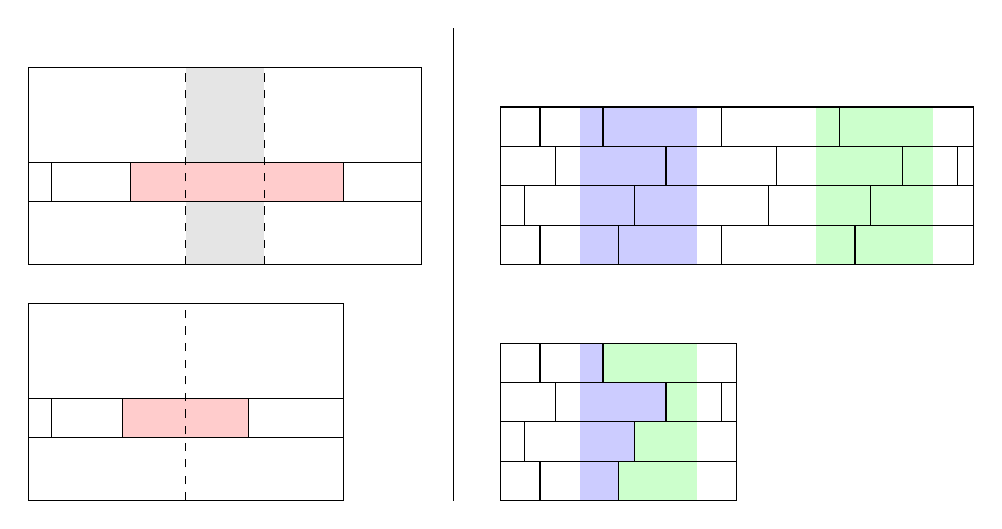
\begin{tikzpicture}
		\draw[white,fill=gray!20] (2,0) rectangle (3,0.8);
		\draw[white,fill=gray!20] (2,1.3) rectangle (3,2.5);
		
		\draw (0,0) rectangle (5,2.5);
		
		\draw (0,0.8) rectangle (5,1.3);
		
		\draw (0,0.8) rectangle (0.3,1.3);
		\draw (0,0.8) rectangle (1.3,1.3);
		\draw[fill=red!20] (1.3,0.8) rectangle (4,1.3);
		
		\draw[dashed] (2,0) -- (2,2.5);
		\draw[dashed] (3,0) -- (3,2.5);
		
		
		
		\draw (0,-3) rectangle (4,-0.5);
		
		\draw (0,-2.2) rectangle (4,-1.7);
		
		\draw (0,-2.2) rectangle (0.3,-1.7);
		\draw (0.3,-2.2) rectangle (1.3,-1.7);
		\draw[fill=red!20] (1.2,-2.2) rectangle (2.8,-1.7);
		
		\draw[dashed] (2,-3) -- (2,-0.5);
		
		\draw (5.4,-3) -- (5.4,3);
		
		
		\draw[white,fill=blue!20] (7,0) rectangle (8.5,2);
		\draw[white,fill=green!20] (10,0) rectangle (11.5,2);
		
		\draw (6,0) rectangle (12,2);
		
		\draw (6,0) rectangle (12,0.5);
		\draw (6,0) rectangle (12,1);
		\draw (6,0) rectangle (12,1.5);
		
		\draw (6,0) rectangle (6.5,0.5);
		\draw (6,0) rectangle (7.5,0.5);
		\draw (6,0) rectangle (8.8,0.5);
		\draw (6,0) rectangle (10.5,0.5);
		
		\draw (6,0.5) rectangle (6.3,1);
		\draw (6,0.5) rectangle (7.7,1);
		\draw (6,0.5) rectangle (9.4,1);
		\draw (6,0.5) rectangle (10.7,1);
		
		\draw (6,1) rectangle (6.7,1.5);
		\draw (6,1) rectangle (8.1,1.5);
		\draw (6,1) rectangle (9.5,1.5);
		\draw (6,1) rectangle (11.1,1.5);
		\draw (6,1) rectangle (11.8,1.5);
		
		\draw (6,1.5) rectangle (6.5,2);
		\draw (6,1.5) rectangle (7.3,2);
		\draw (6,1.5) rectangle (8.8,2);
		\draw (6,1.5) rectangle (10.3,2);
		
		
		\draw[white, fill=blue!20] (7,-3) rectangle (7.5,-2.5);
		\draw[white,fill=blue!20] (7,-2.5) rectangle (7.7,-2);
		\draw[white,fill=blue!20] (7,-2) rectangle (8.1,-1.5);
		\draw[white,fill=blue!20] (7,-1.5) rectangle (7.3,-1);
		
		\draw[white,fill=green!20] (7.5,-3) rectangle (8.5,-2.5);
		\draw[white,fill=green!20] (7.7,-2.5) rectangle (8.5,-2);
		\draw[white,fill=green!20] (8.1,-2) rectangle (8.5,-1.5);
		\draw[white,fill=green!20] (7.3,-1.5) rectangle (8.5,-1);
		
		
		
		\draw (6,-3) rectangle (9,-2.5);
		\draw (6,-3) rectangle (9,-2);
		\draw (6,-3) rectangle (9,-1.5);
		\draw (6,-3) rectangle (9,-1);
		
		\draw (6,-3) rectangle (6.5,-2.5);
		\draw (6,-3) rectangle (7.5,-2.5);
		
		\draw (6,-2.5) rectangle (6.3,-2);
		\draw (6,-2.5) rectangle (7.7,-2);
		
		\draw (6,-2) rectangle (6.7,-1.5);
		\draw (6,-2) rectangle (8.1,-1.5);
		\draw (6,-2) rectangle (8.8,-1.5);
		
		\draw (6,-1.5) rectangle (6.5,-1);
		\draw (6,-1.5) rectangle (7.3,-1);
		
	\end{tikzpicture}


	\caption{Illustration of the proof of Lemma~\ref{lem:short-local-runs}. We represent local runs as above, where Lines correspond to registers, and vertical separations are times at which a $\enregact$ operation is performed on that register. If one register $i$ keeps the same value for a long enough time (on the left), we apply the induction hypothesis to shorten the projection of the run on the other registers. As the value of $i$ does not change, the resulting run is still valid. If all registers change values often, say every $M$ steps (on the right), then if the run is long enough we can find two identical sequences of transitions during which all values are renewed twice. We can then obtain a shorter run by glueing them together as in the picture. The colored rectangles in the shortened runs correspond to fresh values that we introduce to make sure that all local disequality tests succeed.}
\end{figure}
\begin{restatable}{lemma}{lemShortLocalRuns}
	\label{lem:short-local-runs}
	There exists a function $\towerfun(n) (\regnum)$ in $O(\intro*\repexp{n}{\regnum})$ such that, for every protocol $\prot$ with $r$ registers per process, for every "local run" $\localrun: (q, \localdata) \step{*} (q', \localdata')$ in $\prot$, for every $V \subseteq \nats$ finite that contains every message value appearing in $\localrun$, there exists $\localrun': (q, \localdata) \step{*} (q', \localdata')$\corto{uniformiser la notation} such that $\length{\localrun'} \leq \towerfun(\size{\prot})(r)$ and:
	\begin{enumerate}
		\item \label{item:shorterrun_anyvalue} for all $\aval' \in \nats$, there exists $\aval \in \nats$ such that $\vinput{\aval'}{\localrun'}$ is a subword of $\vinput{\aval}{\localrun}$,
		\item \label{item:shorterrun_oldvalues} for all $\aval \in V$, $\vinput{\aval}{\localrun'}$ is a subword of $\vinput{\aval}{\localrun}$. 
		% \item by writing $V := \nats \setminus \set{\localdata_i(k) \mid k \in \nset{1}{\regnum}}$, for every $\aval' \in V$, there exists $\aval \in V$ such that $\vinput{\aval'}{\localrun'}$ is a subword of $\vinput{\aval}{\localrun}$.
	\end{enumerate}
		%  with an "input" $I$.
% 	Let $u_1, u_2, u_3$ be such that $u=u_1u_2u_3$.
% 	If $\size{u_2} > TOWER$, then there exists $u'_2$ with $|u_2'| \leq \towerfun(\prot)$ such that $u_1u'_2u_3$ is a local run of $\prot$ with smaller "input" than $u$. 
\end{restatable}

\begin{remark}
	The tower bound of Lemma~\ref{lem:short-local-runs} is tight, in the sense that some local runs may need to have length a tower of exponentials of linear height in the number of registers.
	It also holds for pushdown automata, and for all transition systems which have some kind of pumping lemma.
	\cortoin{To formalize}
\end{remark}


\begin{restatable}{lemma}{lemShortRunOutput}
	\label{lem:short-run-for-output}
	For every protocol $\prot$ with $r$ registers per process, for every $w_{in} \in (\messages\times \nats)^*$, if there exists a "local run" $\localrun: (q, \localdata) \step{*} (q', \localdata')$ in $\prot$ such that $w_{in} \subword \Output{\localrun}$, then for every $V \subseteq \nats$ finite that contains every message value appearing in $\localrun$, there exists $\localrun': (q, \localdata) \step{*} (q', \localdata')$ such that $\length{\localrun'} \leq (\towerfun(\size{\prot})(r)+1)\size{w_{in}}$, $w_{in} \subword \Output{\localrun'}$ and:
	
	\begin{enumerate}
		\item for all $\aval' \in \nats$, there exists $\aval \in \nats$ such that $\vinput{\aval'}{\localrun'}$ is a subword of $\vinput{\aval}{\localrun}$,
		\item for all $\aval \in V$, $\vinput{\aval}{\localrun'}$ is a subword of $\vinput{\aval}{\localrun}$. 
	\end{enumerate}
\end{restatable}


\begin{restatable}{lemma}{lemBoundSuccessorHeight}
	\label{lem:bound-successor-height}
	Let $\prot$ be a "protocol", let $\node$ be a node of a "tree unfolding" $\tree$ of minimal size labelled by $\prot$ satisfying a "boss specification" $w$.
	Let $\node_1, \ldots, \node_k$ be its "follower" children. If $\node$ is not the root of $\tree$ then let $\mu'$ be its father.
	We have the following properties:
	
	\begin{enumerate}
		\item $k \leq \size{\messages}r$ 
		
		\item The root of $\tree$ is a "boss node".
				
		\item  If $\node$ is a "boss node" then 
		\begin{itemize}
			\item If $\node$ is the root of $\tree$ then $\bosslabel{\node} = w$
			
			\item If $\node$ is not the root then $\size{\bosslabel{\node}} \leq \size{\localrunlabel{\node'}}$
			
			\item In both cases $\size{\localrunlabel{\node}} \leq (\towerfun(\size{\prot})(r) + 1)\Big[ \size{\bosslabel{\node}} + \sum_{i=1}^k \size{\followlabelword{\node_i}} \Big]$
		\end{itemize}
	
		\item If $\node$ is a "follower node" then 
		\begin{itemize}			
			\item $\size{\followlabelword{\node}} \leq \size{\localrunlabel{\node}}$
			
			\item $\size{\localrunlabel{\node}} \leq (\towerfun(\size{\prot})(r) +1)\Big[ 1 + \sum_{i=1}^k \size{\followlabelword{\node_i}} \Big]$
			
		\end{itemize}
	\end{enumerate}
\end{restatable}


\subsection{Tree bounds}
\label{sec:tree-bounds}

\begin{definition}
	We define the ""altitude"" of a node $\node$, written $\altitude{\node}$, in a "tree unfolding" recursively as follows:
	\begin{itemize}
		\item The altitude of the root is $0$
		
		\item The altitude of a "boss node" is the altitude of its father minus one
		
		\item The altitude of a "follower node" is the altitude of its father plus one.
	\end{itemize}
\end{definition}

\begin{restatable}{lemma}{lemBoundLengthHeightH}
	\label{lem:bound-length-at-height-h}
	Let $\prot$ be a protocol, let $\node$ be a node of a "tree unfolding" of minimal size labelled by $\prot$ satisfying a "boss specification" $w$.
	Let $\altmax$ be the maximal "altitude" in $\tau$, let $N = \size{w} + \size{\prot} +1$ and let $f_0 : \nats \to \nats$ be the function mapping each $n \in \nats$ to $f_0(n)=(N^2 (\towerfun(N)(N) + 1))^{n+1}$ 
	
	\begin{itemize}
		\item If $\node$ is a "boss node" then $\size{\bosslabel{\node}} \leq f_0(\altmax - \altitude{\node}-1)$ and $\size{\localrunlabel{\node}} \leq f_0(\altmax - \altitude{\node})$.
		
		\item If $\node$ is a "follower node" then $\size{\localrunlabel{\node}} \leq \size{\followlabelword{\node}} \leq  f_0(\altmax - \altitude{\node})$.
	\end{itemize} 
\end{restatable}

\begin{restatable}{lemma}{lemBoundMaxHeight}
	\label{lem:bound-max-height}
	There exists a function $f_1$ of the class $\Falpha{\omega^{\size{\messages}}}$ such that for all "protocol" $\prot$, for all "tree unfolding" $\tree$ of minimal size labelled by $\prot$ satisfying a "boss specification" $w$, the maximal altitude of a node of $\tree$ is bounded by $f_1(\size{\prot} + \size{w}+1)$.
\end{restatable}


\begin{restatable}{lemma}{lemBoundMinHeight}
	\label{lem:bound-min-height}
	There exists a function $f_2$ of the class $\Falpha{\omega^{\size{\messages}+1}}$ such that for all "protocol" $\prot$, for all "tree unfolding" $\tree$ of minimal size labelled by $\prot$ satisfying a "boss specification" $w$, the absolute value of the minimal "altitude" of a node of $\tree$ is bounded by $f_2(\size{\prot} + \size{w}+1)$.
\end{restatable}



\begin{corollary}
	\label{cor:bound-node-size}
	There exists a function $f_3$ of the class $\Falpha{\omega^{\size{\messages}+1}}$\corto{corriger les M en M+1} such that for all "protocol" $\prot$, for all "tree unfolding" $\tree$ of minimal size labelled by $\prot$ satisfying a "boss specification" $w$, for all node $\node$ of $\tree$,
	
		\begin{itemize}
		\item $\size{\localrunlabel{\node}} \leq f_3(\size{\prot}+ \size{w})$
			
		\item If $\node$ is a "boss node" then $\size{\bosslabel{\node}} \leq f_3(\size{\prot}+ \size{w})$.
		
		\item If $\node$ is a "follower node" then $\size{\followlabelword{\node}} \leq f_3(\size{\prot}+ \size{w})$.
	\end{itemize} 
\end{corollary}

\ifproofs
\begin{proof}
	Consequence of Lemmas~\ref{lem:bound-length-at-height-h}, \ref{lem:bound-max-height} and \ref{lem:bound-min-height} as $\Falpha{\omega^{\size{\messages}}}$ is closed by composition with elementary functions.
\end{proof}
\fi
\begin{restatable}{proposition}{PropBoundTreeSize}
	\label{prop:bound-tree-size}
	There exists a function $f_4$ of the class $\Falpha{\omega^{\size{\messages}+1}}$ such that for all "protocol" $\prot$, for all "tree unfolding" $\tree$ of minimal size labelled by $\prot$ satisfying a "boss specification" $w$, the size of $\tree$ is bounded by $f_4(\size{\prot} + \size{w}+1)$.
\end{restatable}




\subsection{Decidability}
\label{sec:decidability-end}

\begin{theorem}
	The BNRA coverability problem is decidable in time $\Falpha{\omega^\omega}$ and there is no $\alpha < \omega^\omega$ such that this problem can be solved in time $\Falpha{\alpha}$.
	The lower bound holds even with two registers and no local tests.
\end{theorem}

\ifproofs
\begin{proof}
	The lower bound is given by the reduction from "lossy channel systems" reachability in Proposition~\ref{prop:reduction-LCS} and by the fact that there is no algorithm in time $\Falpha{\alpha}$ for LCS reachability with $\alpha < \omega^\omega$.
	
	For the upper bound, let $\prot$ be a "protocol" with $\regnum \geq 1$ registers over messages $\messages$ and $q$ one of its states. We add a new message $m$ to $\messages$ and a new transition $\br{m}{1}$ from $q$ to itself broadcasting $m$. 
	Clearly the new "protocol" $\prot'$ satisfies the "boss specification" $m$ if and only if $q$ is coverable in $\prot$.
	
	By Lemmas~\ref{lem:run-to-tree} and \ref{lem:tree-to-run}, there is a run of $\prot'$ satisfying $m$ if and only if there is a "tree unfolding" satisfying $m$.
	By Lemma~\ref{prop:bound-tree-size}, there is such a "tree unfolding" if and only if there is one of size at most $f_4(\size{\prot}+2)$, where $f_4$ is a function of the class $\Falpha{\omega^{\size{\messages}}}$.
	
	The last problem we have is that the size of a "tree unfolding" does not take into account the values used in it. This can be solved by noticing that the conditions in the definition of a "tree unfolding" and the condition to satisfy a "specification" still hold after applying an injective renaming to the values. 
	
	Suppose there exists $\tree$ a "tree unfolding" satisfying $m$, let $V$ be the set of values appearing in that tree. In a node $\node$ the values appearing are $\valuelabel{\node}$, the initial values of $\localrunlabel{\node}$ (there are $r$ such values), the non-initial values (at most $\size{\localrunlabel{\node}}$ as they all need to be received).
	Hence there are at most $\size{\localrunlabel{\node}} + r +1$ different values appearing in each node.
	In total there are thus at most $\sum_{\node \in \tree} \size{\localrunlabel{\node}} + r +1$ different values in $\tree$, which is less than $(r+2)\size{\tree}$.
	
	We can apply an injective renaming $V \to \nset{1}{(r+2)\size{\tree}}$ to the values to obtain another "tree unfolding" satisfying $m$ and whose values do not exceed $(r+2)\size{\tree}$.
	As a result, there exists a "tree unfolding" satisfying $m$ if and only if there is one of size at most $f_4(\size{\prot}+2)$ in which values do not exceed $f_4(\size{\prot}+2)$. A description of such a tree requires a space that is polynomial in its size.
	
	We can therefore bound the size of the description of such a "tree unfolding" by a function of $\Falpha{\omega^{\size{\messages}}}$.
	An algorithm for the coverability problem thus consists in enumerating all trees labelled by local runs of $\prot$ of size at most $f_4(\size{\prot}+2)$ with values not exceeding $f_4(\size{\prot}+2)$, and accepting if and only if one of them satisfies the conditions to be a "tree unfolding" satisfying $m$.
	This can all be done in exponential time in $f_4(\size{\prot}+2)$, thus this algorithm terminates in time $f_5(\size{\prot})$ where $f_5$ is a function of $\Falpha{\omega^{\size{\messages}}}$.
	
	The BNRA coverability problem is thus decidable in time $\Falpha{\omega^\omega}$.
\end{proof}
\fi
